\chapter{Background}

This chapter provides the necessary background required to understand the results of the comparative studies presented in subsequent chapters. A description of the design and operation of the representative virtualization platforms is presented, followed by a discussion of a simplified version of the Intelligent River\textsuperscript{\textregistered} middleware architecture.

\section{Virtualization Technologies}
%\chapter{Virtualization Technologies}
The accelerated adoption of Linux in the cloud computing ecosystem has spurred the demand for dynamic, efficient, and flexible ways to virtualize next-generation workloads. Not surprisingly, there is no single best solution to satisfy such a demand. The Linux community supports multiple mature virtualization platforms, leaving the choice to end-users. This chapter provides a technical overview of the principles behind the operation of three representative virtualization solutions: Kernel-based Virtual Machines (KVM), Xen, and Linux Containers.

%General introduction about virtualization. What types of virtualization we are going to talk in this thesis. Introduce LXC, KVM, Xen.
%Write about the technical background behind all three.
%specifically, LXC is an userspace wrapper over the linux containers facility merged into the Linux kernel.
%The idea of KVM and its isolation benefits as it allows running individual kernels for the VMs.
%The fundamental idea of para virtualization on which Xen is based on.

\subsection{Kernel-based Virtual Machines (KVM)}
%\section{Kernel based Virtual Machines (KVM)}

KVM is representative of a category of virtualization solutions known as \emph{full-virtualization}. A full-virtualization solution, as shown in Figure \ref{img_full_virt}, is one where a set of virtual devices are emulated over a set of physical devices, with a \emph{hypervisor} to arbitrate access from the \emph{virtual machines}, sometimes referred to as \emph{guests}.


%Block diagram of a full-virtualization system%\includegraphics[width=110mm]{../../Pictures/full-virt.png} 
\begin{figure}[htbp]
\centering
\includegraphics[width=120mm]{full-virt.png}
\caption{A Full-Virtualization System}
\label{img_full_virt}
\end{figure}
A hypervisor is a critical part of a stable operating environment. It is responsible for managing the memory available to the guests, scheduling the processes, managing the network connections to and from the guests, managing the input/output facilities, and maintaining security. The KVM solution, being a relatively new entrant into the virtualization scene, chose to build upon existing utilities and features by leveraging the mature, time-proven Linux kernel to perform the role of the hypervisor. 

In the KVM-based approach to virtualization, the majority of the work is offloaded to the Linux kernel, which exposes a robust, standard, and secure interface to run isolated virtual machines. The virtualization facilities enabled by KVM were merged into the mainstream Linux kernel since version 2.6.20 (released February 2007) \cite{kvm_linux_kernel}. KVM itself is only part of the virtualization solution. It turns the Linux kernel into a Virtual Machine Monitor (VMM) (i.e, hypervisor), which enables several virtual machines to operate simultaneously, as if they were running on their own hardware. KVM uses an independent tool known as QEMU \cite{qemu} to create virtual devices for the virtual machines. Hence, the total solution is commonly referred to as QEMU-KVM. KVM is packaged as a lightweight kernel module which implements the virtual machines as regular Linux processes, and therefore leverages the Linux kernel on the host for all scheduling and device management activities. 
Figure \ref{img_kvm_arch} shows the architecture of a server virtualized using QEMU-KVM. A server with a virtualization capable processor, disk storage, and network interfaces runs a standard Linux operating system that contains KVM. Virtual machines co-exist with the user-space applications running directly on the host. The virtual machines contain a set of virtual devices created using QEMU and run an unmodified guest operating system like Linux or Microsoft Windows.

%\newpage 
\begin{figure}[htbp]
\centering
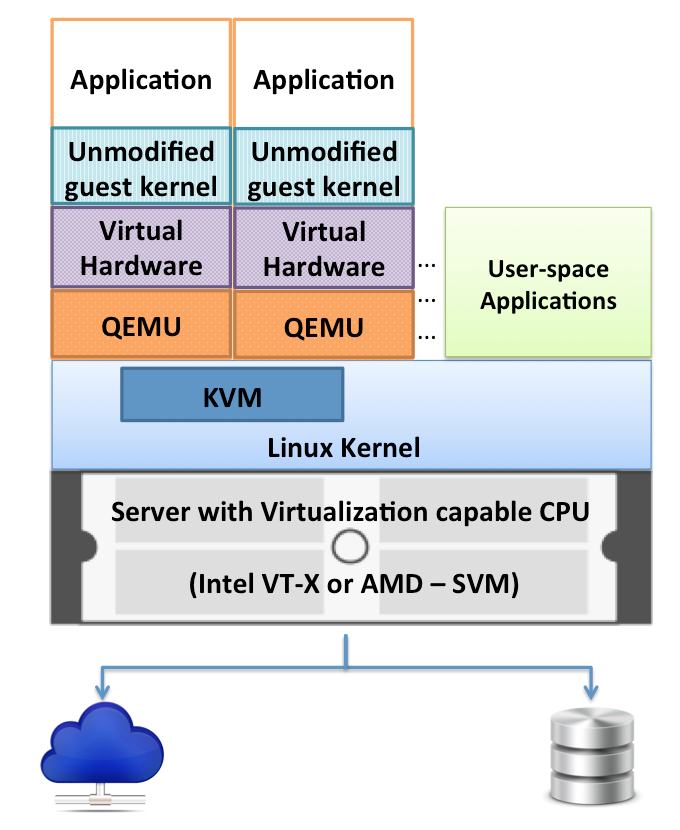
\includegraphics[width=120mm]{kvm-arch.png}
\caption{KVM - Architecture}
\label{img_kvm_arch}
\end{figure}

In practice, KVM and the Linux kernel treat the virtual machines as regular Linux processes and perform the mapping of virtual devices to real devices in each of the following categories.

\begin{enumerate}
\item \textbf{CPU}:

KVM requires the CPU to be virtualization-aware. 
%\begin{wrapfigure}{r}{0.5\textwidth}[htbp]
  %\begin{center}
\begin{figure}[htbp]
\centering
    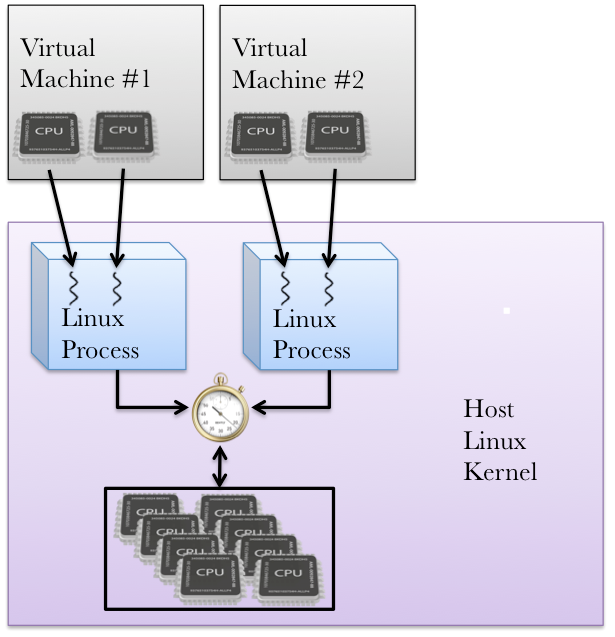
\includegraphics[width=0.48\textwidth]{kvm-cpu.png}
  %\end{center}
  \caption{KVM - Virtual CPU Management}
  \label{img_kvm_thread}
\end{figure}
%\end{wrapfigure}
Intel VT-X \cite{intelvtx} and AMD-SVM \cite{amdv} are the virtualization extensions provided by Intel and AMD, respectively, which are the most common CPUs used in x86-based servers. KVM relies on these facilities to isolate the instructions generated by the guest operating systems from those generated by the host itself. Every virtual CPU associated with a virtual machine is created as a thread belonging to the virtual machine's process on the host, as shown in Figure \ref{img_kvm_thread}. Hence, enabling multiple virtual CPUs improves the virtual machine's performance by utilizing the multi-threading facilities on the host. The virtual machine's CPU requests are scheduled by the host kernel using the regular CPU scheduling policies. Improving CPU performance on the guest and ensuring fair CPU entitlement are discussed in later chapters.   

\item \textbf{Memory}:

KVM inherits the memory management facilities of the Linux kernel. The memory of a virtual machine is an abstraction over the virtual memory of the standard Linux process on the host. This memory can be swapped, shared with other processes, merged, and  otherwise managed by the Linux kernel. Thus, the total memory associated with all the virtual machines on a host can be greater than the physical memory available on the host. This feature is known as \emph{memory over-commitment}. Though memory over-commitment increases overall memory utilization, it creates performance problems when all the virtual machines try to utilize their memory share at the same time, leading to swapping on the host. Since KVM offloads memory management to the Linux kernel, it enjoys the support of NUMA (Non-Uniform Memory Access) awareness \cite{numa}, and Huge Pages \cite{huge_pages} to optimize the memory allocated to the virtual machines. NUMA support is discussed in chapter 6.
   
\item \textbf{Network Interfaces}:

Networking in a virtualized infrastructure enables an additional layer of convenience and control over conventional networking practices. Virtual machines can be networked to the host, among each other, or even participate in the same network segment as the host. Several configurations are possible, trading-off device compatibility and performance.\begin{figure}
        \centering
        \begin{subfigure}[b]{0.35\textwidth}
                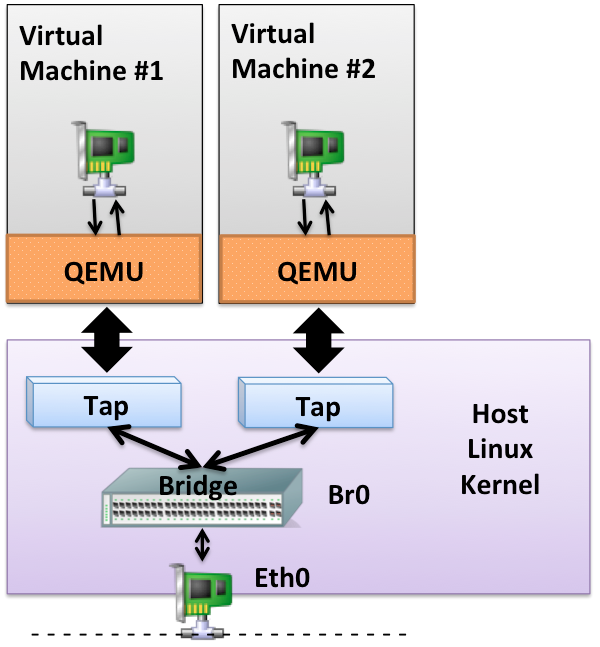
\includegraphics[width=\textwidth]{kvm-emulated.png}
                \caption{Emulated Networking Devices}
                \label{fig:kvm-emulated}
        \end{subfigure}%
        ~ %add desired spacing between images, e. g. ~, \quad, \qquad etc.
        \qquad \hspace{8 mm}
          %(or a blank line to force the subfigure onto a new line)
        \begin{subfigure}[b]{0.35\textwidth}
                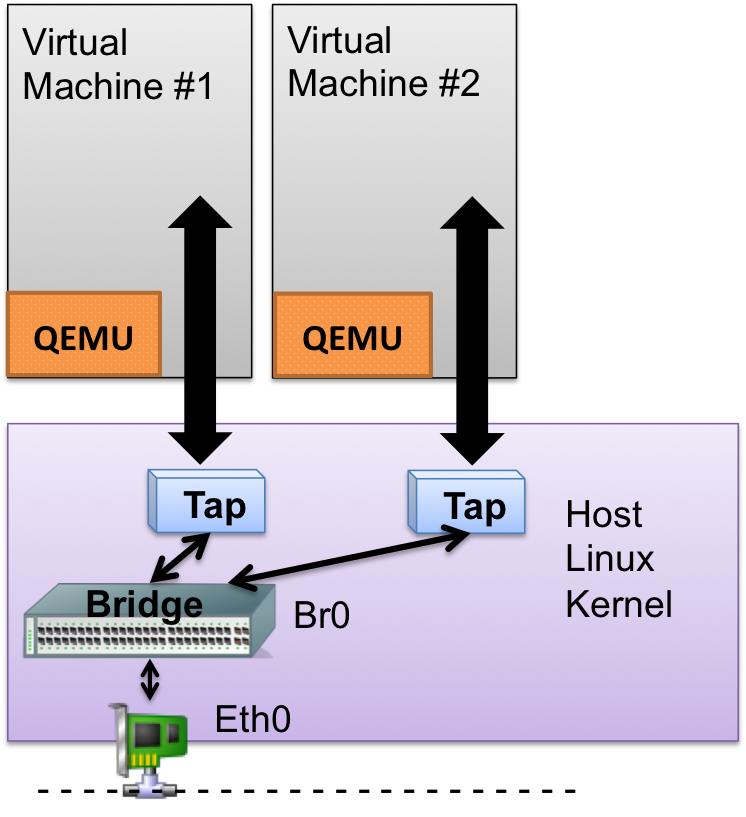
\includegraphics[width=\textwidth]{kvm-para.png}
                \caption{Para-Virtualized Networking}
                \label{fig:kvm-para}
        \end{subfigure}
        ~ %add desired spacing between images, e. g. ~, \quad, \qquad etc.
\newline \newline
          %(or a blank line to force the subfigure onto a new line)
        \begin{subfigure}[b]{0.35\textwidth}
                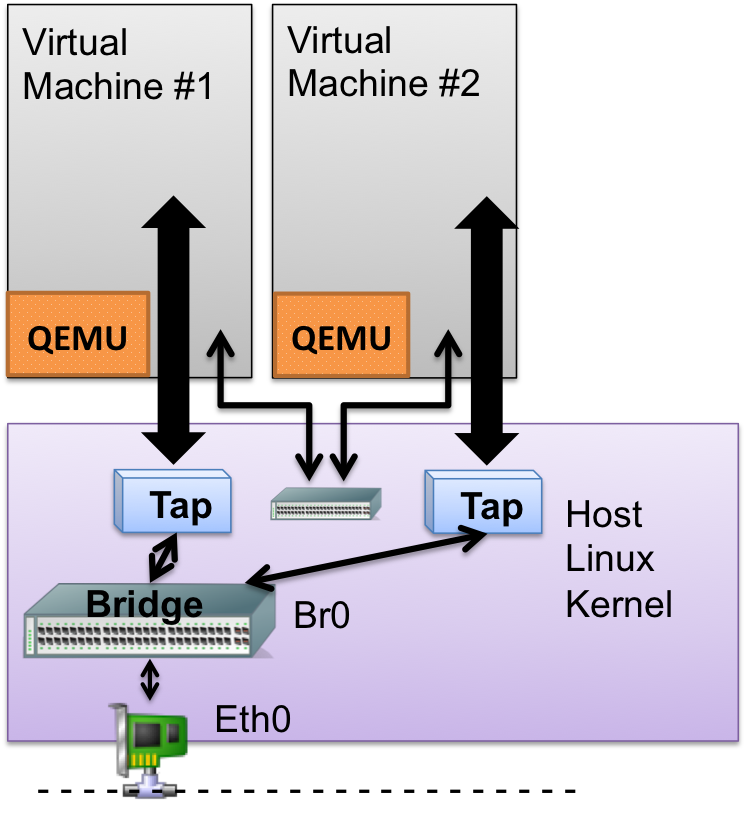
\includegraphics[width=\textwidth]{kvm-internal.png}
                \caption{Public and Private Networking}
                \label{fig:kvm-internal}
        \end{subfigure}
        \quad \hspace{8 mm}
        \begin{subfigure}[b]{0.35\textwidth}
                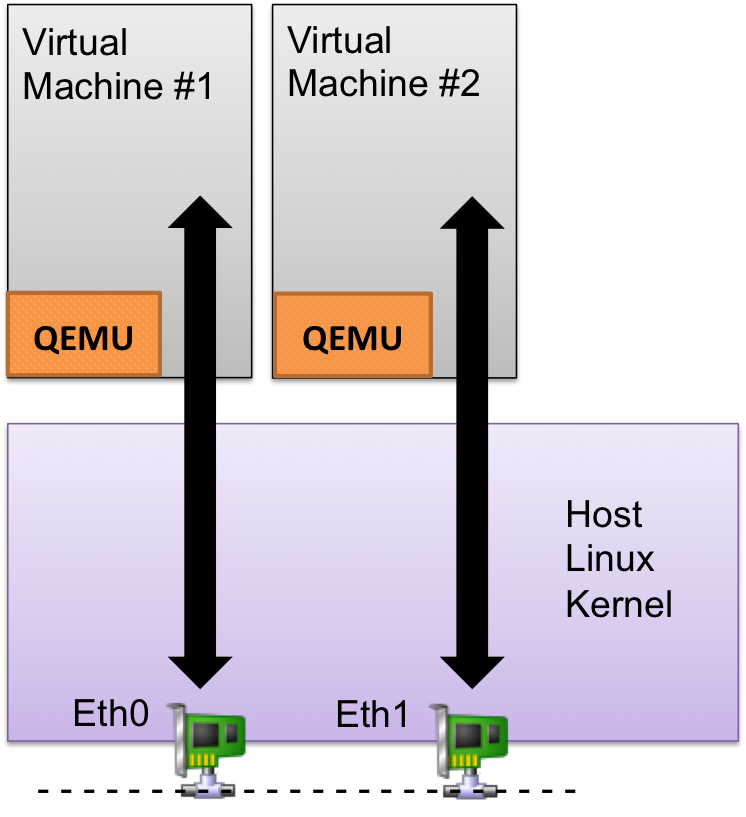
\includegraphics[width=\textwidth]{kvm-direct.png}
                \caption{Direct Device Assignment}
                \label{fig:kvm-direct}
        \end{subfigure}
\newline \newline
        \begin{subfigure}[b]{0.42\textwidth}
                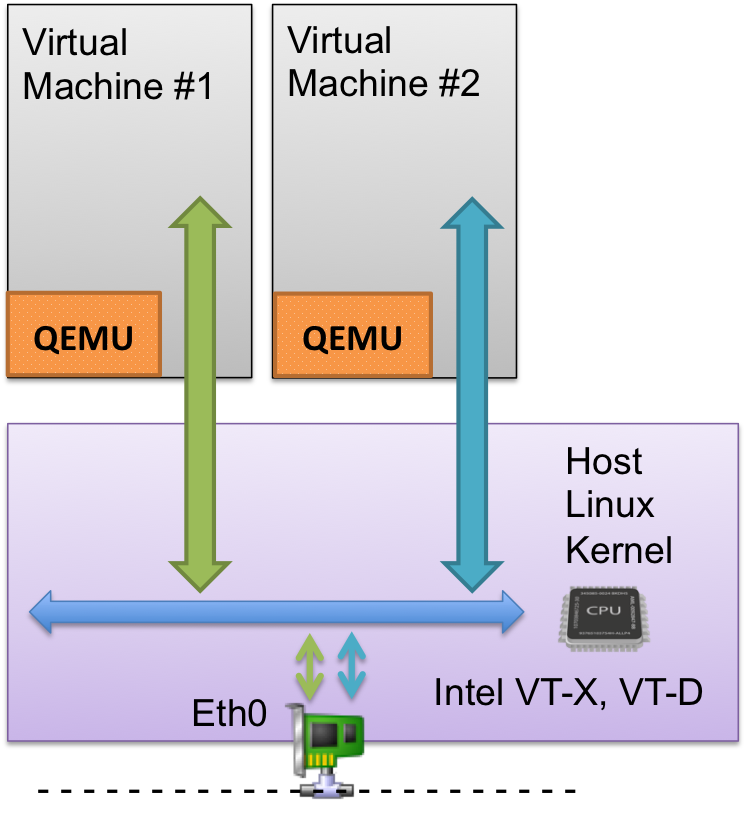
\includegraphics[width=\textwidth]{kvm-direct-sriov.png}
                \caption{Direct Device Assignment with SR-IOV}
                \label{fig:kvm-direct-sriov}
        \end{subfigure}
        \caption{Common Networking Options for KVM}\label{fig:kvm-networking}
\end{figure} Figure \ref{fig:kvm-networking} shows the most common virtual networking options used in KVM-based infrastructure. Figure \ref{fig:kvm-emulated} shows a virtual networking configuration where unmodified guest operating systems use their native drivers to interact with their virtual network devices. Virtual network devices are connected to the Tap devices \cite{Tap_devices} on the host kernel. Tap interfaces are software-only interfaces existing only in the kernel; they relay ethernet frames to and from the Linux bridge. This setup trades performance to achieve superior device compatibility.



Figure \ref{fig:kvm-para} shows a networking configuration where the guest operating system running in the virtual machine is ``virtualization aware'' and cooperates with the host by bypassing the device emulation provided by QEMU. This is known as \emph{para-virtualized networking}. Para-virtualized networking trades compatibility to achieve near-native performance.



Figure \ref{fig:kvm-internal} shows a combination of both public and private networking. Two points are important to note. First, a virtual machine may have multiple virtual networking devices. Second, virtual machines can be privately networked using a Linux bridge that is not backed by a physical ethernet device. This setup greatly increases the inter-virtual machine communication performance as the packets need not leave the server to pass through real networking hardware. This is an ideal networking configuration for a publicly accessible virtual machine to communicate with secure private virtual machines. For example, a publicly accessible application server could then communicate with a privately networked database server.



To support the virtualization of network-intensive applications, physical network interfaces attached to the host can be directly assigned to the virtual machines, bypassing the host kernel and QEMU, as shown in Figure \ref{fig:kvm-direct}. This setup provides ``bare-metal'' performance by providing direct access to the hardware, applicable when individual hardware devices are available to be dedicated to the virtual machines. The key to achieving this direct device access is the hardware assistance provided through Intel VT-D \cite{intelvtd}, and AMD-IOMMU \cite{amd-iommu}. Intel VT-D and AMD-IOMMU enable secure PCI-pass through to allow the guest operating system in the virtual machine to control the hardware on the host.



Figure \ref{fig:kvm-direct-sriov} shows a networking setup that utilizes ethernet hardware capable of Intel Single Root Input/Output Virtualization (SR-IOV) \cite{sr-iov_primer}. SR-IOV takes the above configuration one step further by letting a single hardware device be accessed directly by multiple virtual machines, with their own configuration space and interrupts. This enables a capable network card to appear as several virtual devices, capable of being directly accessed by multiple virtual machines.


\textbf{Advanced Networking: }  Virtual LANs (VLANs) provide the capability to create logically separate networks that share the same physical medium. In a virtualized environment, VLANs created for the virtual machines may share the physical network interfaces or share the bridged interface.


\end{enumerate}

% ********** TO DO *****************

\subsection{Linux Containers}
%\section{Linux Containers}

%Linux Containers are a lightweight operating system virtualization technology. virtualization with Containers is the newest entrant into the linux virtualization arena. There is also an interesting perspective from the Linux community that hypervisors originated due to the linux kernel's incompetence to provide superior resource isolation and effective scale \cite{linux_incompetent} and Containers are the way for the linux kernel to fix them. The core idea is to isolate only a set of processes and their resources in \emph{"Containers"} without involving any device emulation or creating any dependency on the host hardware. Like virtual machines, several containers can run simultaneously on a single host, but all of them share the host kernel for their operation. Isolated containers run directly on the bare-metal hardware using the device drivers native to the host kernel without any intermediate relays. 


%The idea of containers is not new. Solaris Zones [cite], BSD Jails [cite], and Chroot have been around for a long time and are considered as the predecessors for Linux Containers. BSD Jails were designed with an objective of restricting the visibility of the host's resources to a process. For example, when a process runs inside a jail, its root directory is changed to a sub-directory on the host thereby limiting the extent of the file system the process can access. Each process in a jail is provided its own directory sub tree, an IP address defined as an alias to the interface on the host, and optionally a hostname that resolves to its own IP address.

%Linux Containers expanded the scope of BSD jails, and provides a granular operating system virtualization platform to the extent where, containers can be isolated from each other running their own operating system yet sharing the kernel with the host. Containers are provided their own independent file system and network stack. Every container can run its own linux distribution of linux that is different from the host. For example, a host server running RedHat Enterprise Linux [cite] may run containers that run Debian [cite], Ubuntu [cite], CentOS [cite] etc. or even another copy of RedHat Enterprise Linux. This level of abstraction in the containers create an illusion of running virtual machines as discussed earlier with KVM.  

%\begin{figure}[htbp]
%\centering
%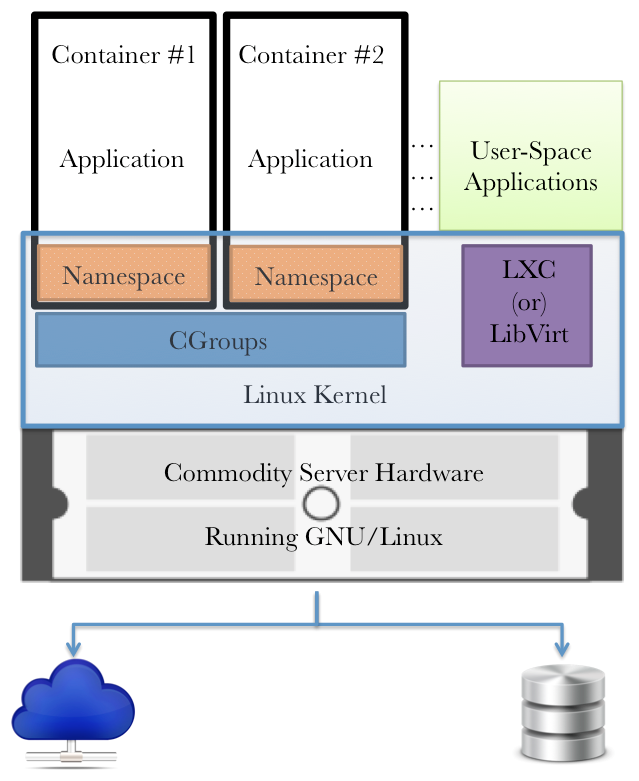
\includegraphics[width=130mm]{lxc-arch.png}
%\caption{Linux Containers - Architecture}
%\label{img_lxc_arch}
%\end{figure}

%Figure \ref{img_lxc_arch} shows the architecture of a server that uses linux containers for virtualization. Unlike KVM, linux containers does not require any assistance from the hardware therefore runs on any hardware that is capable of running the mainline linux kernel. The linux kernel facilitates the execution of containers by the implementation of namespaces at various levels. write about lxc architecture, namespaces, cgroups and that user space applications can co-exist.




Linux Containers are a lightweight operating system virtualization technology and the newest entrant into the Linux virtualization arena. There is an interesting perspective popularized within the Linux community that hypervisors originated due to the Linux kernel's inability to provide superior resource isolation and effective scalability \cite{linux_incompetent}. Containers are the proposed solution. Digging deeper, hypervisors were created to isolate workloads and create virtual operating environments, with individual kernels optimally configured in accordance with workload requirements. The key question to be answered is
\emph{whether it is the responsibility of an operating system to flexibly isolate its own workloads.}
If the Linux kernel could solve this problem without the overhead and complexity of running several individual kernels, there would not be a need for hypervisors!


The Linux community saw a partial solution to this problem in BSD Jails \cite{jails}, Solaris Zones \cite{zones}, Chroot \cite{chroot}, and most importantly, OpenVZ \cite{openvz} - a fork of the Linux kernel maintained by Parallels. BSD Jails were designed to restrict the visibility of the host's resources from a process. For example, when a process runs inside a jail, its root directory is changed to a sub-directory on the host, thereby limiting the extent of the filesystem the process can access. Each process in a jail is provided its own directory sub tree, an IP address defined as an alias to the interface on the host, and optionally, a hostname that resolves to the jail's own IP address. 

The Linux kernel's approach to solving the resource isolation problem is \emph{``Containers''}, incorporating the benefits of the above mentioned inspirations and more. The core idea is to isolate a set of processes and their resources in containers, without involving any device emulation or imposing virtualization requirements on the host hardware. Like virtual machines, several containers can run simultaneously on a single host, but all of them share the host kernel for their operation. Isolated containers run directly on the bare-metal hardware using the device drivers native to the host kernel without any intermediate relays. 


Containers expand the scope of BSD jails, providing a granular operating system virtualization platform, where containers can be isolated from each other, running their own operating system, yet sharing the kernel with the host. Containers are provided their own independent file system and network stack. Every container can run its own distribution of Linux that may be different from the host, but must use the host's kernel instead of its own. For example, a host server running RedHat Enterprise Linux \cite{rhel} may run containers that run Debian \cite{debian}, Ubuntu \cite{ubuntu}, CentOS \cite{centos}, etc., or even another copy of RedHat Enterprise Linux. This level of abstraction in the containers creates an illusion of running virtual machines, as discussed earlier with KVM.  

\begin{figure}[H]
\centering
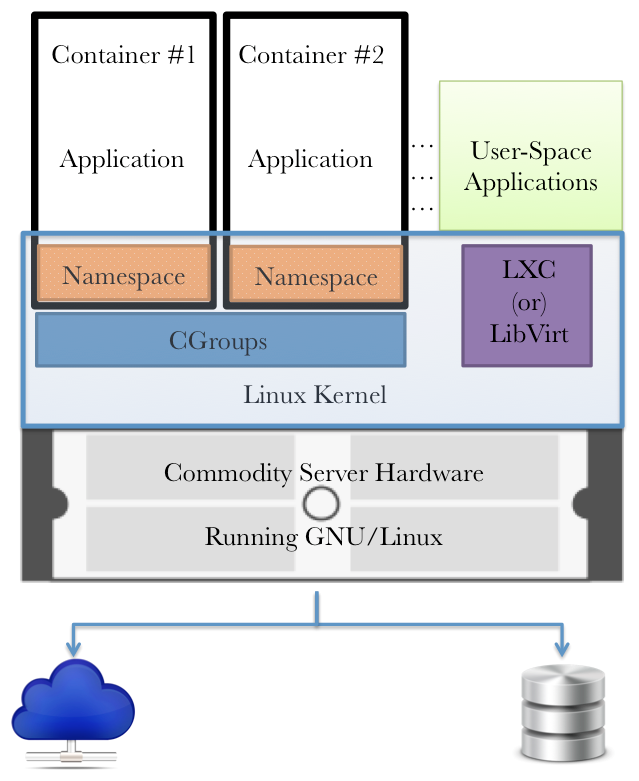
\includegraphics[width=110mm]{lxc-arch.png}
\caption{Linux Containers - Architecture}
\label{img_lxc_arch}
\end{figure}

Figure \ref{img_lxc_arch} shows the architecture of a server that uses Linux Containers for virtualization. Unlike KVM, Linux Containers do not require any assistance from the hardware; the solution can run on any platform capable of running the mainline Linux kernel. The kernel facilitates the execution of containers by utilizing \emph{namespaces} for resource isolation, and \emph{cgroups} for resource management and control. Containers can be administered using the standard libvirt API and the LXC suite of command line tools. Since containers are viewed as regular Linux process groups by the Linux kernel, they can coexist with any user-space applications that may be running directly on the physical server. 

\newpage
The following description of namespaces in the Linux kernel is based on \cite{namespaces1}, \cite{namespaces2}, \cite{namespaces3}, \cite{namespaces4}, \cite{namespaces5}, and \cite{namespaces6}.
%A synopsis of the implementation of namespaces in the linux kernel described by Michael Kerrisk in [cite], [cite], [cite], [cite] :-
%The inclusion of namespaces into the linux kernel was described in detail by Michael Kerrisk through a series of articles. The following discussion on various namespaces at various levels. write about lxc architecture, namespaces, cgroups and that user space applications can co-exist.
Namespaces ``wrap'' a global system resource on the host and make it appear to the processes within the namespace (containers) as though they have their own isolated instance of the global resource. Linux implements 6 types of namespaces: 
\begin{itemize}
\item \textbf{Mount namespaces :}

Mount namespaces enable isolated file system trees to be associated with specific containers (or groups of regular Linux processes). A container can create its own file system setup, and the subsequent \textit{mount()} and \textit{unmount()} system calls issued by the process affect only its mount namespace, instead of the whole system. For example, multiple containers on the same host can issue \textit{mount()} calls to create a mount point ``/data'', and access the mount points at ``/data'' simultaneously. They will reside at different locations on the filesystem tree, e.g., ``/\textless containername1\textgreater /data'', ``/\textless containername2\textgreater /data'', and so on. Of course, the same setup can be achieved using the \textit{chroot()} command, but \emph{chroot} can be escaped with certain capabilities, including CAP\_SYS\_CHROOT \cite{capabilities}. Mount namespaces provide a secure alternative. They also improve portability, as each container can retain its filesystem tree, regardless of the host's environment.


\item \textbf{UTS namespaces :}

UNIX Time-sharing System (UTS) namespaces facilitate the use of the \textit{sethostname()} and \textit{setdomainname()} system calls to set the container hostname and NIS domain name, respectively. \textit{uname()} returns the appropriate hostname and domain names.


\item \textbf{IPC namespaces :}

IPC namespaces isolate the System V IPC objects \cite{sysv_ipc} and POSIX message queues \cite{posix_msg_queues} associated with individual containers.


\item \textbf{PID namespaces :}

PID namespaces in the Linux kernel facilitate the isolation of process identification numbers (PIDs) associated with processes running on the host and within its containers. Every container can have its own init process (PID 1). In general, several containers running simultaneously can have processes with identical PIDs. The Linux kernel implements the PIDs as a structure consisting of two numeric PIDs, one in the container's namespace, and the other outside the namespace (i.e., in the host kernel). This PID abstraction is useful in two regards. First, it isolates the containers such that a process running in one container does not have visibility into processes running in other containers. Second, it enables the migration of containers across hosts, as the containers can retain the same PIDs.


\item \textbf{Network namespaces :}

Network namespaces provide isolation of network resources for containers, enabling the containers to have their own (virtual) network devices, IP addresses, port numbers, and IP routing tables. For example, a single host can run multiple containers, each running a web server at its own IP address over port 80.


\item \textbf{User namespaces :}

User namespaces provide isolation for user and group IDs. Each process has two user and group IDs, one inside the container's namespace, and the other outside the namespace. This enables a user to possess a UID of 0 (root privileges) inside a container, while still being treated as an unprivileged user on the host. The same applies to application processes that run inside the containers. This abstraction of user privilege greatly improves the security of container-based virtualization solutions. It should be noted that this feature is only available in Linux kernel versions 3.8+.
\end{itemize}


Four new namespaces are being developed for future inclusion in the Linux kernel \cite{linux_namespaces_plan}:


\begin{itemize}

\item \textbf{Security namespace :} This namespace aims to provide isolation of security policies and security checks among containers.

\item \textbf{Security keys namespace :} This namespace aims to provide an independent security key space for containers to isolate the /proc/keys and /proc/key-users files based on the namespace \cite{key_namespace}.

\item \textbf{Device namespace :} This namespace aims to provide each container its own device namespace to enable containers to create/access devices with their own major and minor numbers so they can be seamlessly migrated across hosts.

\item \textbf{Time namespace :} This namespace aims to enable containers to freeze/modify their thread and process clocks, which would support ``live'' host migration. 
\end{itemize}




Control groups (cgroups) \cite{cgroups} \cite{cgroups-rami-rosen} \cite{cgroups-redhat} are another key feature of the Linux kernel, used to allocate resources such as CPU, memory, network bandwidth, and disk access bandwidth among user-defined groups of processes (containers). cgroups instrument the Linux kernel to limit, prioritize, monitor, and isolate system resources. With proper usage of cgroups, hardware and software resources on the host can be efficiently allocated and shared among several containers. cgroups can be dynamically re-configured and made persistent across reboots of the host. Though cgroups are generic and apply to individual processes and process groups, the remainder of this section discusses their relavance to containers.

The implementation of cgroups categorizes manageable system resources into the following subsystems : 

%\newline
\begin{table}[h!]
\begin{center}
\renewcommand{\arraystretch}{2.0}
\begin{tabular}{ | p{1.5cm} | p{12.5cm} | }
  \hline                 
  \textbf{Cpu} & Used to set limits on CPU access for containers \\ \hline       
  \textbf{Cpuset} & Used to confine containers to system subsets of CPUs and memory (“memory nodes”) \\ \hline
  \textbf{Cpuacct} & Used to track the usage of CPU resources by containers in a cgroup \\ \hline
  \textbf{Memory} & Used to set limits on memory use by containers in a cgroup \\ \hline
  \textbf{Blkio} & Used to set limits on input/output access to and from block devices \\ \hline
  \textbf{Devices} & Used to allow or deny access to devices by containers in a cgroup \\ \hline
  \textbf{Net\_cls} & Used to tag network packets with a class identifier (classid) that allows the Linux Traffic Controller (tc) to identify packets originating from a particular cgroup task \\ \hline
  \textbf{Net\_prio} & Used to prioritize the network traffic to and from containers on a per network interface basis \\ \hline
\end{tabular}
\end{center}
\caption{cgroups - Subsystems}
\end{table}
%\begin{enumerate}

%
%\item \textbf{blkio} : Allows to set limits on input/output access to and from block devices such as physical drives.
%
%
%\item \textbf{cpu} : Allows to set limits on the access to the CPU for the tasks (Containers).
%
%
%\item \textbf{cpuacct} : Reporting the usage of CPU resources by tasks/containers in a cgroup.
%
%
%\item \textbf{cpuset} : Enables assignment of individual CPUs (on a multicore system) and memory nodes to tasks/containers in a cgroup.
%
%
%\item \textbf{devices} : Allows or denies access to devices by tasks/containers in a cgroup.
%
%
%\item \textbf{freezer} : This subsystem suspends or resumes tasks in a cgroup.
%    
%    
%\item \textbf{memory} : Allows setting limits on memory use by tasks/containers in a cgroup, and generates automatic reports on memory resources used by them.
%    
%    
%\item \textbf{net\_cls} : This subsystem tags network packets with a class identifier (classid) that allows the Linux traffic controller (tc) to identify packets originating from a particular cgroup task.
%
%
%\item \textbf{net\_prio} : Enables prioritizing the network traffic to and from the tasks/containers on a per network interface basis.
%
%
%\item \textbf{ns} : The namespace subsystem. 
%
%\end{enumerate}
%

cgroups are organized hierarchically. There may be several hierarchies of cgroups in the host system, each associated with at least one subsystem. Process groups (in our case, containers) are assigned to cgroups in different hierarchies to be managed by different subsystems. All the containers in the Linux system are a member of the root cgroup by default and are associated with custom, user-defined cgroups on an as-needed basis.

\begin{figure}[H]
\centering
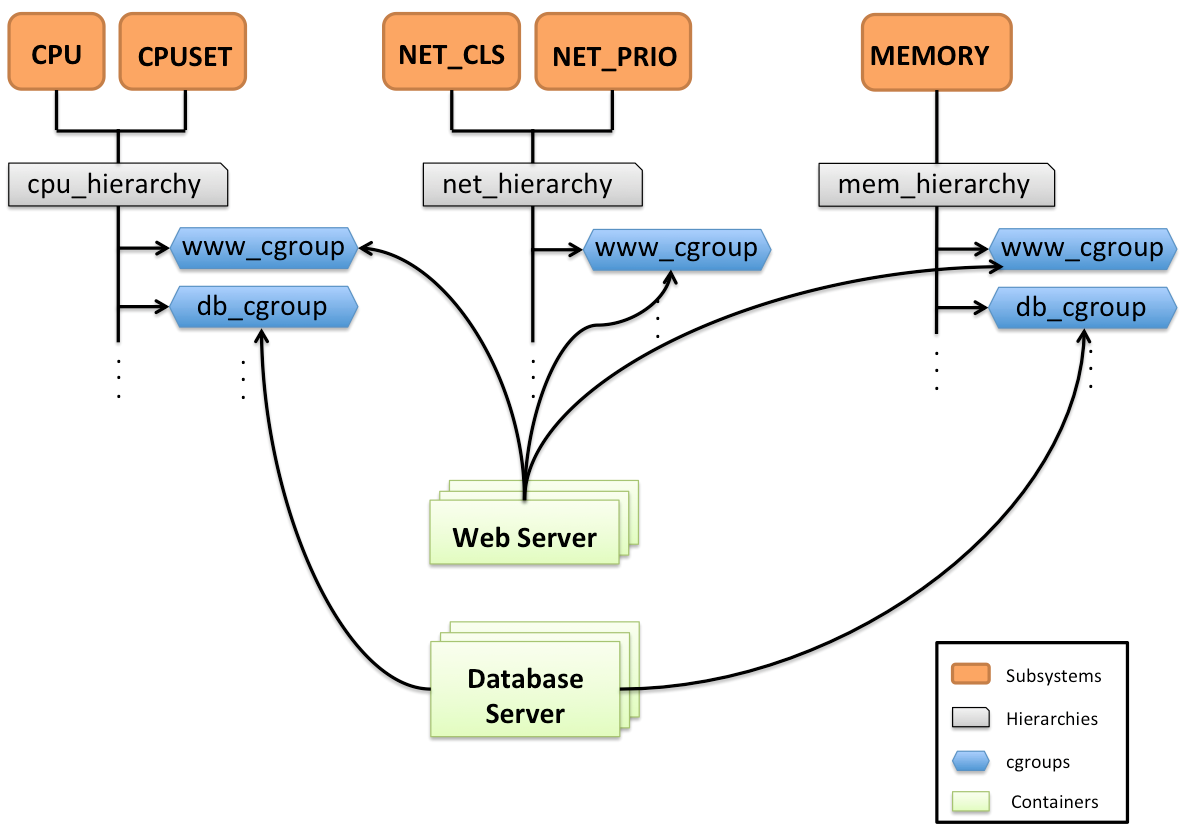
\includegraphics[width=\textwidth]{cgroup-example.png}
\caption{cgroups Example Configuration}
\label{img_cgroup_example}
\end{figure}

Figure \ref{img_cgroup_example} shows an example configuration of cgroups for a system running multiple web and database servers within containers. The objective is to limit the CPU, network bandwidth, and memory available to each container based on whether it runs a web server or a database server. First, a hierarchy is created for the type(s) of subsystem(s) required. For example, mem\_hierarchy is created with an association to the memory subsystem. Second, custom cgroups are created under the hierarchy based on the anticipated workload categories. For example, www\_cgroup is created to define policies for all the containers that run a web server. The kernel automatically populates the cgroup’s directory with the required settings. Third, limits are set on the created cgroup. For example, the amount of memory available to all containers associated with a cgroup can be set to 2 gigabytes. Finally, all the containers that are provisioned to run a web server are added to the respective cgroup -- in our example, www\_cgroup. 

The approach discussed above may be repeated for different subsystems (e.g. CPU, blkio) to limit the corresponding resources. In the example shown in Figure \ref{img_cgroup_example}, all the containers running a web server are associated with the cgroup, www\_cgroup, which limits their resource usage in terms of memory, network bandwidth, and CPU time. All containers running a database server are associated with db\_cgroup, which limits their usage in terms of memory and CPU utilization, while allowing them to use unlimited network bandwidth. 






%
%The configuration of cgroups are governed by a basic set of rules :-
%
%\begin{itemize}
%
%
%\item A single hierarchy can have one or more subsystems attached to it.
%
%\item A subsystem can have several hierarchies that are not already associated with any other subsystems.
%
%\item A container can be assigned to several cgroups but, cannot belong to more than one cgroup in the same hierarchy.
%
%\item The future children of all the processes within a container will inherit the same cgroup associations from their parent process. However their cgroup associations may be changed independantly while in execution.
%
%\end{itemize}
%
%
%Adhering to the above mentioned rules makes sure that, there is exactly one way a container is controlled by a single subsystem. 
%
%
%\begin{figure}[htbp]
%\centering
%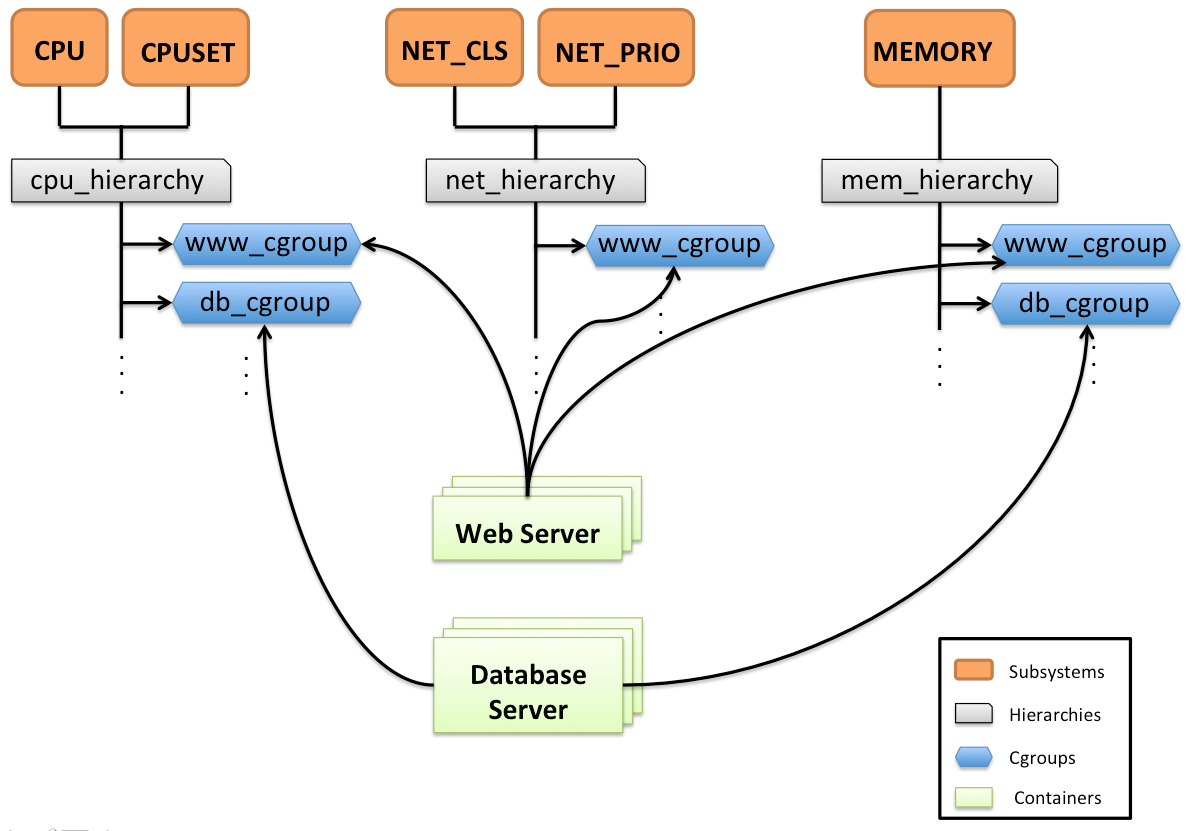
\includegraphics[width=\textwidth]{cgroup_example.png}
%\caption{Cgroups configuration example}
%\label{img_cgroup_example}
%\end{figure}
%
%
%
%Figure \ref{img_cgroup_example} shows an example to illustrate the configuration of cgroups. Containers running web servers are assigned the cgroup that specifies appropriate limits on the resources(CPU, network and memory) it requires. The cgroups are in turn assigned to individual hierarchies which are  with the appropriate subsystems (type of resource that is to be managed). Containers running as database servers are limited/managed only for CPU and memory, while using network resources like any other process in the system.
%
%
%Chapter <??> describes cgroups in more detail as part of the resource entitlement discussion.  


%  ******************** TO DO   *****************************

% Write about networking facilities available for lxc containers ... refer this blog.    http://l3net.wordpress.com/2013/08/25/debian-virtualization-lxc-network-isolation/


%Write about sharing common binaries among the containers for smaller footprint and more performance. 

%Write about the relevance of union filesystems (layered operation) and journaled file systems (Easy Snapshotting) and mention CRIU project that allows checkpointing and restart of Linux processes(Containers) that bring live migration to linux containers.

%Another innovative perspective upon the idea of containers is coreOS - google more.

\subsection{Xen}
%\section{Xen}


Xen \cite{xen_overview} is an open source virtualization platform that provides a bare-metal hypervisor implemented as special firmware that runs directly on the hardware. The Xen project is based on para-virtualization \cite{paravirt}  \cite{paravirt1}, a technique where guest operating systems are modified to run on the host using an interface that is easier to virtualize. Para-virtualization significantly reduces overhead and improves performance \cite{paravirt}, \cite{art_of_virt}, \cite{xen_perf}.

\begin{figure}[H]
\centering
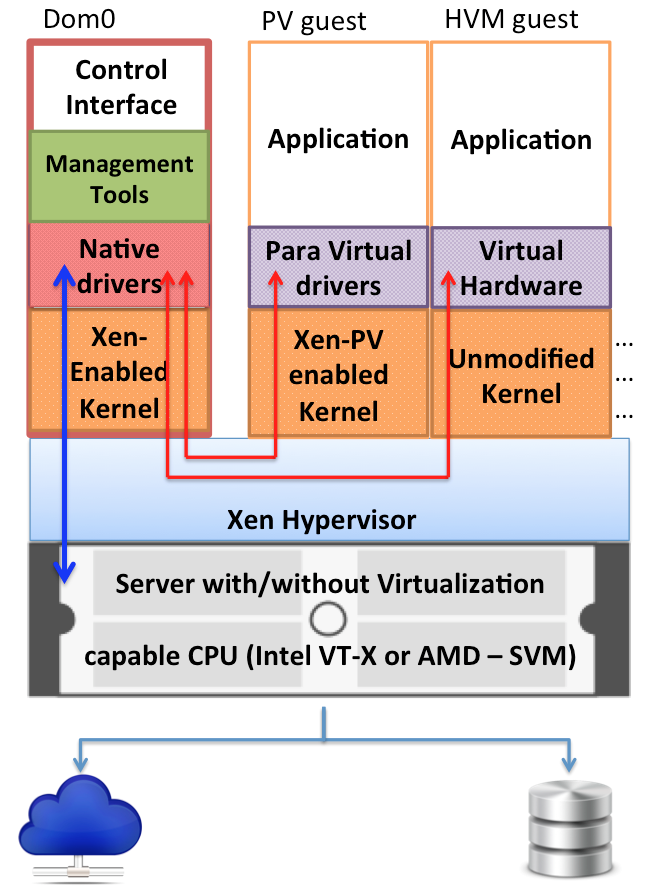
\includegraphics[width=90mm]{xen-arch.png}
\caption{Xen - Architecture}
\label{xen_arch}
\end{figure}

The architecture of a system virtualized using Xen is shown in Figure \ref{xen_arch}. 
The Xen hypervisor runs directly from the bootloader. The hypervisor is also referred to as the \emph{Virtual Machine Monitor (VMM)}; it is responsible for managing CPU, memory, and interrupts. The virtual machines, referred to as \emph{domains} or \emph{guests}, run on top of the hypervisor. A special domain referred to as \emph{domain0} acts as a controller, containing the drivers for all the devices in the system. domain0 accesses the hardware directly, interacting with the other domains, and acts as the control interface for administrators to control the entire system. This controller domain also contains the set of tools to create, configure, and destroy virtual machines. It runs a modified version of the Linux kernel that can perform the role of Controller \cite{dom0_kernels}. All other domains are totally isolated from the hardware and can use these resources only through the controller; they are referred to as \emph{unprivileged domains (DomU)}. The DomUs can be either para-virtualized (PV) or hardware-assisted (HVM). The para-virtualized guests can run only modified operating systems, as they require a Xen-PV-enabled kernel and PV drivers, which make them aware of the hypervisor. As an upside, para-virtualized guests do not require the CPUs to have virtualization extensions, and are usually lightweight compared to the unmodified operating systems.  HVM guests can run unmodified operating systems, but require virtualization extensions on the CPU, just like KVM. The HVM guests use QEMU to emulate virtual hardware to provide the unmodified guest operating system. Both para-virtualized guests and hardware-assisted guests can run on a single system at the same time. Recent work on the Xen project also attempts to utilize the para-virtualized drivers on a HVM guest to improve performance, combining the best of both solutions.


\section{Intelligent River\textsuperscript{\textregistered} Middleware}

Intelligent River\textsuperscript{\textregistered} is an ongoing interdisciplinary research initiative at Clemson University that aims to deploy a highly distributed ecological sensor network in the Savannah River Basin. Specially designed sensor nodes measure various ecological factors and transmit observations to a real-time Intelligent River\textsuperscript{\textregistered} Middleware system. The middleware system is responsible for (i) performing semantic analysis of the real-time observation stream, (ii) reliably persisting the observations, and (iii) publishing the processed observations in multiple formats for further analysis and visualization. The comparative study presented in this thesis was motivated by a need to identify the most suitable virtualization platform to virtualize the constituent middleware components. Here we briefly  introduce the architectural model of the Intelligent River\textsuperscript{\textregistered} middleware system and describe the operational characteristics of its components to set the context for the comparative studies presented in subsequent chapters.

\begin{figure}[htbp]
\centering
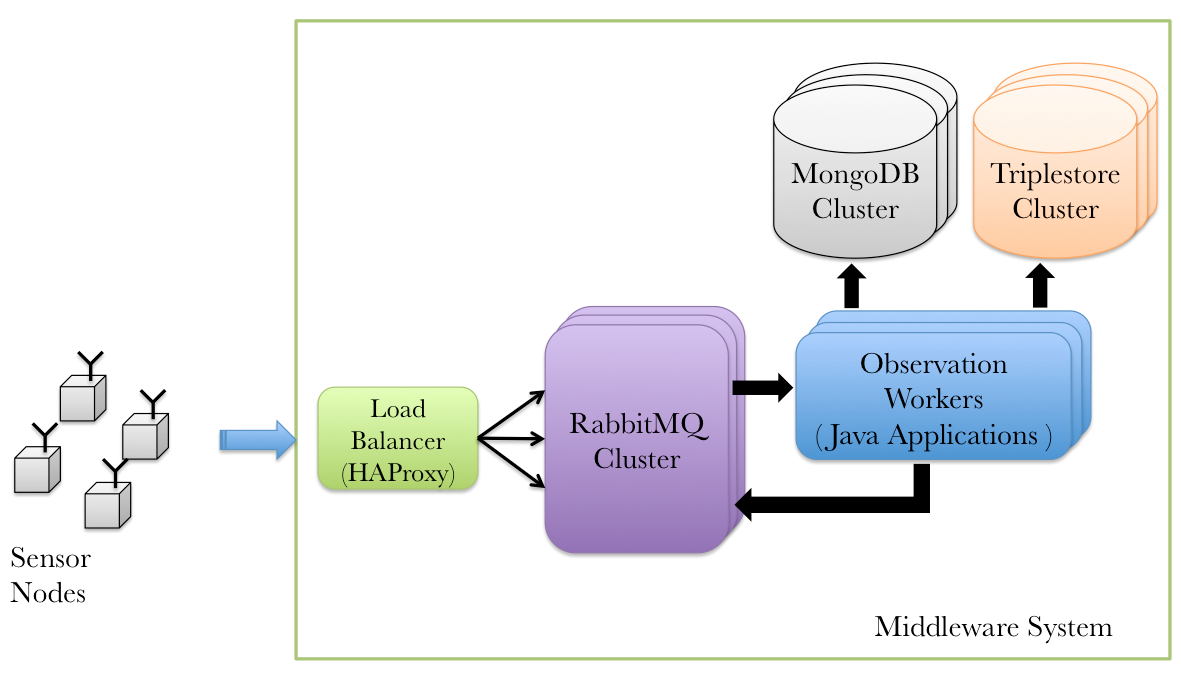
\includegraphics[width=130mm]{ir.png}
\caption{Simplified Architectural Model of the Intelligent River\textsuperscript{\textregistered} Middleware System}
\label{fig:ir}
\end{figure}

Figure \ref{fig:ir} shows a simplified version of the Intelligent River\textsuperscript{\textregistered} Middleware architecture. \emph{Sensor nodes} are custom-designed hardware devices known as \emph{MoteStacks} \cite{ir}. The \emph{Load balancer} is an open source TCP load-balancing application, HAProxy \cite{haproxy} running on a physical server. The \emph{RabbitMQ cluster} comprises of multiple instances of an open source message broker, RabbitMQ \cite{rabbitmq}. The \emph{observation workers} are custom developed Java applications, each deployed on a physical server. The \emph{MongoDB cluster} comprises of multiple instances of MongoDB \cite{mongodb}, setup in a sharded configuration \cite{mongosharding}. The \emph{Triplestore cluster} comprises of multiple instances of Apache Jena TDB \cite{jenatdb}.

Sensor nodes gather data from commodity sensor probes and transmit the collected observations to the load balancer through multiple networks, both wired and wireless. The load balancer relays the observations to any of the servers in the RabbitMQ cluster, which queues the observations to be fetched by  observation workers. Worker applications fetch the queued observations from the message queues in the RabbitMQ cluster and perform (i) semantic analysis on the observations, (ii) persist both processed and unprocessed  observations to MongoDB, (iii) persist the processed observations to a triplestore, and (iv) publish the processed observations back to RabbitMQ for further analysis and visualization. The architecture of the middleware system is based on a hybrid of message queuing, client-server, and publish/subscribe patterns. Such an architecture yields a system with components that are loosely coupled, enabling them to scale independently based on demand. If the middleware system receives observations at a rate higher than the existing set of observation worker applications can process, additional instances can be commissioned on new servers to fetch and process observations off the queues, improving overall system throughput. Similarly, the MongoDB cluster is setup using a sharded configuration, so that new servers, each running MongoDB, can be added as shards to the existing cluster based on demand. The triplestore cluster is also designed so that new servers, each running Apache Jena TDB, can be added to the cluster on an as-needed basis.

Given the loosely coupled configuration and the dynamically changing demands of the middleware system, it serves as an ideal candidate to leverage the benefits of a virtualized infrastructure.   



%The key differences in ideology of Xen as against the earlier discussed KVM, are :-
%\begin{itemize}
%\item Ability to run fully para-virtualized guests that have been optimized to run as a virtual machine.
%
%
%\item Ability to run para-virtualized guests even on CPUs without any hardware assistance.
%
%
%\item Lightweight hypervisor compared to the full linux kernel being used as hypervisor with KVM.
%
%
%\item Claims of better security as (i) The drivers run on a virtual machine instead of the hypervisor (ii) Reduced attack surface due to the smaller footprint of the hypervisor compared to the linux kernel. 
%
%
%\item Though not widely used,  Operating systems other than linux, NetBSD and OpenSolaris can be used to run the controller VM (Dom0).
%
%\end{itemize}






%Same as the above two .. A good technical introduction, followed by a block diagram and more detailed explanation.

%\begin{figure}[htbp]
%\centering
%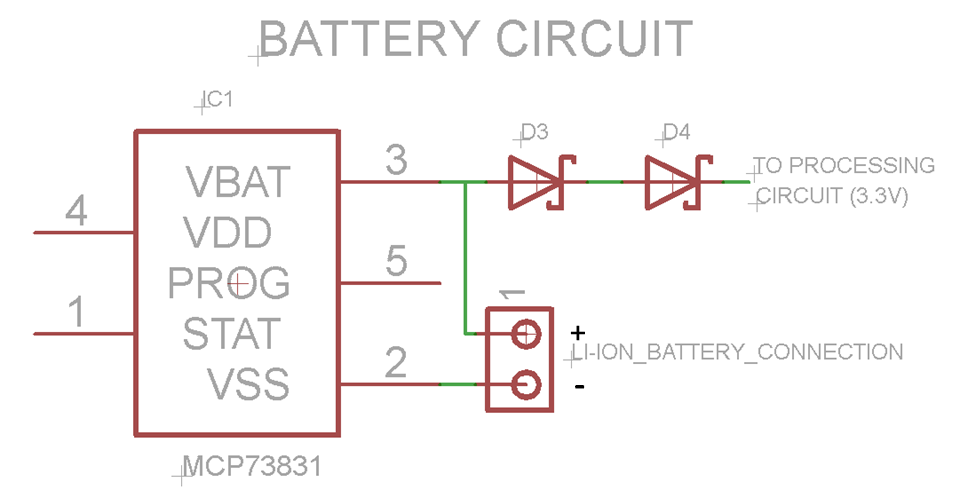
\includegraphics[width=\columnwidth]{battery_ckt.PNG}
%\caption{Battery Circuit}
%\label{img_batteryCircuit}
%\end{figure}
%
%As shown in Figure \ref{img_batteryCircuit}, 